\documentclass[12pt,leqno]{article}

\usepackage{indentfirst}

\usepackage{graphicx}
\graphicspath{ {./img/} }

\textwidth              16 cm
\textheight             23 cm
\oddsidemargin          -1 cm
\evensidemargin         -1 cm
\topmargin              -1 cm
\setlength{\evensidemargin}{15.5pt}
\setlength{\oddsidemargin}{2.5pt}

\pagestyle{empty}

\def\ClasaO{{\mathcal O}}

\usepackage{array}
\newcolumntype{P}[1]{>{\centering\arraybackslash}p{#1}}

\usepackage{multirow}
\usepackage{subcaption}
\usepackage{hyperref}

\usepackage{pgfplots}
\pgfplotsset{width=5in,compat=1.9}

\title{How a genetic algorithm change when using gray coding}
\author{Stamate Valentin 2B4}

\begin{document}

\maketitle

\section*{Abstract}

  In this raport we will see how the results change when using gray coding for gene instead of binary.

\section{Introduction}
  We already saw how good a genetic algorithm is when it comes on solving an optimization problem that cannot be solved using a deterministic algorithm because of the complexity.
  This time, we will try to see if we can make it better by introducing adaptive parameters and changing the codification of the gene from binary to gray.

\subsection{Motivation}
  If the new algorithm gives better results this can have a huge inpact in any different application when genetic algorithm are used, because this adds more flexibility and every algorithm can be
  optimized to fit better in different enviroments.

\section{Methods}
  
  The algorithm used is a genetic algorithm that has adaptive parameters. These are the crossover probability that increses linear with the number of generations 
  $20\%$ in the beginning and $100\%$ at the end. Same for the mutation probability but decreases from $10\%$ to $0.1\%$. Also the number of generation differs together with the input size.
  This will be shown in the result tables.
  
  For every generation the candidates are picked in such a way that the best of them are selected for the next generation keeping the population number constant. 
  
  The genome is reprezented as a bitstring that contains all the components for a point, because the mutations can be made very easy and we work with data.
  Now, instead of using binary codification for gene, we will use gray coding to see what differs.
  For having a slightly time improvement, every codification of a point is kept into an $int$ with the use of binary operators(xor, or, etc).

  The fitness for every candidate is calculated this way $ P(i).fit = pow(10 , 1 / ( - min(P) * cd + F(P(i).gene) + 100) \cdot 2000 + 1) $ where, $ cd $ is 1 if $ min(P) $ 
  is negative, 0 otherwise $min(P)$ is the minimum value found within members, $P$ is the population and $F(gene)$ is the value of the function with the point as a bitstring. 
  This way we keep a positive fitness even if the function takes negative numbers and we don't need to know the global minimum.
  
  The stop condition is when the maximum number of generations is reached.

  Another change is the introduction of a new mutation method described as follows: for 10 members of the population when the mutation happens, 
  we will change the bit only if the fitness is better. This way, those members will only improve in the current generation.


\section{Experimental Setup}
  To have a better idea of how the algorithm is behaving we use different inputs and functions: as function dimention 2, 5, 10, 30 and functions: \href{http://www.geatbx.com/docu/fcnindex-01.html#P89_3085}{\textbf{DeJong's function}}, \href{http://www.geatbx.com/docu/fcnindex-01.html#P150_6749}{\textbf{Schwefel's function}},
  \href{http://www.geatbx.com/docu/fcnindex-01.html#P140_6155}{\textbf{Rastrigin's function}} and \href{http://www.geatbx.com/docu/fcnindex-01.html#P204_10395}{\textbf{Michalewicz's function}}. 
  Each function have a different number of global minimums. The precision for the experiment is 3 so $ \varepsilon = 0.001 $.
  The number of iterations is the same number as the stop condition witch is 500, 1000, 5000 and 7000 iterations/generations and the sample size is 30.

  CPU : Intel i5 - 8265U with 4 phisical and 8 virtual cores.

  Software: Visual Studio Code

  Programming Language: C++ 11

  The reprezentation of the functions have two dimensions and below evey image is the funtion definition, the interval and the global minimum.
  
  \begin{figure}[bp!]
    \centering
    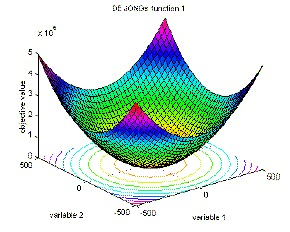
\includegraphics[width=0.4\linewidth, height=5cm]{dejong.jpg} 
    \caption*{De Jong's function: $ f_n(x) = \sum_{i=1}^{n} i x_i^2 $ $\; -5.12 \leq x_i \leq -5.12 $, $\; f(x) \geq 0 $}
  \end{figure}
  
\vfill

\begin{figure}[bp!]
  \centering
  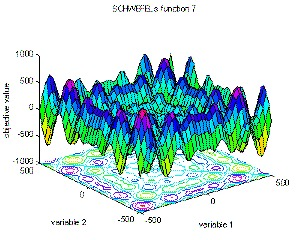
\includegraphics[width=0.4\linewidth, height=5cm]{schwefel.jpg}
  \caption*{Schwefel's function: $ f_n(x) = \sum_{i = 1}^{n}-x_i sin(\sqrt{|x_i|}) , -500 \leq x_i \leq 500 , f_n(x) \geq -n * 418.9829$}
\end{figure}
    
\newpage
\vfill

\begin{figure}[bp!]
  \centering
  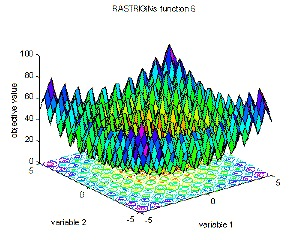
\includegraphics[width=0.4\linewidth, height=5cm]{rastrigin.jpg} 
  \caption*{Rastrigin's function: $ f_n(x) = 10n + \sum_{i = 1}^{n}(x_i^2 - 10 cos(2 \pi x_i)), -5.12 \leq x_i \leq 5.12, f(x) \geq 0 $}
\end{figure}
    
\begin{figure}[bp!]
  \centering
  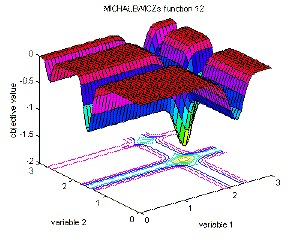
\includegraphics[width=0.4\linewidth, height=5cm]{michalenwicz.jpg}
  \caption*{Michalewicz's function: $ f_n(x) = -\sum_{i = 1}^{n} sin(x_i) (sin(i x_i^2 / \pi)) ^ 20, f_5(x) \geq -4.687, f_{10}(x) \geq -9.66$}  
\end{figure}

\vfill
\clearpage

\section{Results and Comparisons}

% 2
\begin{center}
  \begin{tabular}{|p{2.3cm}||p{3cm}|p{2cm}|p{2cm}|p{4.3cm}|} 
    \hline
    \multicolumn{5}{|c|}{2 dimensions | 500 generations} \\
    \hline
    Function    & Best Value & Mean & StDev & Duration \\ 
    \hline\hline
    De Jong     & $ 0 $ & $ 0 $ & $ 0 $ & 1m 39s \\ 
    \hline
    Schwefel    & $ -837.966 $ & $ -837.9658 $ & $ 0.00042 $ & 3m 36s \\ 
    \hline
    Rastrigin   & $ 0 $ & $ 0.29848 $ & $ 0.48061 $ & 2m 48s \\ 
    \hline
    Michalewicz & $ -0.80132 $ & $ -0.80132 $ & $ 0 $ & 2min 37s \\ 
    \hline
 \end{tabular}
\end{center}

% 5
\begin{center}
  \begin{tabular}{|p{2.3cm}||p{3cm}|p{2cm}|p{2cm}|p{4.3cm}|} 
    \hline
    \multicolumn{5}{|c|}{5 dimensions | 1000 generations} \\
    \hline
    Function    & Best Value & Mean & StDev & Duration \\ 
    \hline\hline
    De Jong     & $ 0 $ & $ 0 $ & $ 0 $ & 15m 33s \\ 
    \hline
    Schwefel    & $ -2094.91 $ & $ -2094.91 $ & $ 0 $ & 21m 25s \\ 
    \hline
    Rastrigin   & $ 0 $ & $ 2.17882 $ & $ 1.79351 $ & 15m 38s \\ 
    \hline
    Michalewicz & $ -3.69885 $ & $ -3.67422 $ & $ 0.05153 $ & 15m 18s \\ 
    \hline
 \end{tabular}
\end{center}

% 10
\begin{center}
  \begin{tabular}{|p{2.3cm}||p{3cm}|p{2cm}|p{2cm}|p{4.3cm}|} 
    \hline
    \multicolumn{5}{|c|}{10 dimensions | 5000 generations} \\
    \hline
    Function    & Best Value & Mean & StDev & Duration \\ 
    \hline\hline
    De Jong     & $ 0 $ & $ 0 $ & $ 0 $ & 2h 12m \\ 
    \hline
    Schwefel    & $ -4189.83 $ & $ -4166.142 $ & $ 49.93869 $ & 3h 3m \\ 
    \hline
    Rastrigin   & $ 0 $ & $ 3.78084 $ & $ 2.13909 $ & 2h 15m \\ 
    \hline
    Michalewicz & $ -8.53593 $ & $ -6.63260 $ & $ 5.376 $ & 2h 10m \\ 
    \hline
 \end{tabular}
\end{center}

% 30
\begin{center}
  \begin{tabular}{|p{2.3cm}||p{3cm}|p{2cm}|p{2cm}|p{4.3cm}|} 
    \hline
    \multicolumn{5}{|c|}{30 dimensions | 7000 generations} \\
    \hline
    Function    & Best Value & Mean & StDev & Duration \\ 
    \hline\hline
    De Jong     & $ 0 $ & $ 0 $ & $ 0 $ & 9h 31m \\ 
    \hline
    Schwefel    & $ -12332.6 $ & $ -12010.84 $ & $ 195.4222 $ & 14h 6m \\ 
    \hline
    Rastrigin   & $ 14.9246 $ & $ 25.27198 $ & $ 6.5697 $ & 10h 39m \\ 
    \hline
    Michalewicz & $ -26.8394 $ & $ -26.22901 $ & $ 0.49174 $ & 9h 33min \\ 
    \hline
 \end{tabular}
\end{center}


\begin{center}
  \resizebox*{9cm}{9cm}{
    \begin{tikzpicture}
      \begin{axis}[
          title={Standard Deviation for Rastrigin's function},
          xlabel={Input [the number of components]},
          ylabel={Value},
          xmin=0, xmax=30,
          ymin=0, ymax=7,
          xtick={0, 2, 5, 10, 30},
          ytick={0, 10, 20, 30},
          legend pos=north west,
          ymajorgrids=true,
          grid style=dashed,
      ]
      
      \addplot[
          color=red,
          mark=square,
          ]
          coordinates {
          (2, 0.48)(5, 1.79)(10, 2.13)(30, 6.56)
          };
          \addlegendentry{Function Evolution}
          
      \end{axis}
    \end{tikzpicture}
  }
\end{center}

 Let's compare this algorithm with the standard one, and also without adaptive parameters.

\begin{center}
  \begin{tabular}{|p{5cm}||p{3cm}|p{2cm}|p{2cm}|} 
    \hline
    \multicolumn{4}{|c|}{Rastrigin's function with 5 dimensions | 1000 generations} \\
    \hline
    Type    & Best Value & Mean & StDev \\ 
    \hline\hline
    $ current $ & $ 0 $ & $ 2.17882 $ & $ 1.79351 $ \\ 
    \hline
    $ without \; adaptive \; par. \; $ & $ 0.0077 $ & $ 0.05781 $ & $ 0.0337 $ \\ 
    \hline
    $ second \; mutation \; $ & $ 0 $ & $ 7.16436 $ & $ 4.93696 $ \\ 
    \hline
    $ old \; approach $ & $ 0.81863 $ & $ 7.84385 $ & $ 3.28231 $ \\ 
    \hline
 \end{tabular}
\end{center}
 
The third result is obtain with the second mutation applied to all members. More than that, the number of dimensions is 30 for that row.

\section{Conclusions}
  We see that the genetic algorithm with adaptive parameters and gray coding gives better results than the standard algorithm with
  binary coding. The mutation probability and crossover variation gives more flexibility so every generic algorithm can be optimized
  to fit better in problems.

\newpage

\begin{thebibliography}{9}
  \bibitem{}
    Return vector of pointers from function \\
    \url{https://stackoverflow.com/questions/39102028/how-to-return-vector-of-pointers-and-ownership-c11}
  \bibitem{}
    Constant size vector \\
    \url{https://stackoverflow.com/questions/11134497/constant-sized-vector}
  \bibitem{}
    Sort a vector of objects \\
    \url{https://stackoverflow.com/questions/1380463/sorting-a-vector-of-custom-objects}  
  \bibitem{}
    Genetic algorithm site \\
    \url{https://profs.info.uaic.ro/~eugennc/teaching/ga/}  
  \bibitem{}
    Coding Train GA playlist \\
    \url{https://www.youtube.com/watch?v=9zfeTw-uFCw&list=PLRqwX-V7Uu6bJM3VgzjNV5YxVxUwzALHV&ab_channel=TheCodingTrain}  
  \bibitem{}
    Seminar 5 notes
  \bibitem{}
    De Jong's function \\
    \url{http://www.geatbx.com/docu/fcnindex-01.html#P89_3085}
  \bibitem{}
    Schwefel's function \\
    \url{http://www.geatbx.com/docu/fcnindex-01.html#P150_6749}
  \bibitem{}
    Rastrigin's function \\
    \url{http://www.geatbx.com/docu/fcnindex-01.html#P140_6155}
  \bibitem{}
    Michalewicz's function \\
    \url{http://www.geatbx.com/docu/fcnindex-01.html#P204_10395}

  \bibitem{}
    Benefits Of Coding Gray \\
    \url{https://stackoverflow.com/questions/41245917/what-are-the-benefits-of-gray-code-in-evolutionary-computation}
  \bibitem{}
    Converting Binary To Gray \\
    \url{https://www.youtube.com/watch?v=cbmh1DPPQyI}
  \bibitem{}
    Gray To Binary \\
    \url{https://www.geeksforgeeks.org/gray-to-binary-and-binary-to-gray-conversion/}
  \bibitem{}
    Second Homework Results

  \end{thebibliography}  
  


\end{document}